%%% LaTeX-Vorlage Version 1.8 %%%

% Grundlegende Dokumenteneigenschaften gemäß DHBW-Vorgaben
\documentclass[a4paper,fontsize=11pt,oneside,parskip=half,headings=normal]{scrreprt} 
% \usepackage{showframe} % nur für Kontrolle der Ränder 

%%% Präambel einbinden (mit Festlegungen gemäß DHBW-Vorgaben) %%%
%%% Präambel %%%
% hier sollten keine Änderungen erforderlich sein
%
\usepackage[utf8]{inputenc}   % Zeichencodierung UTF-8 für Eingabe-Dateien
\usepackage[T1]{fontenc}      % Darstellung von Umlauten im PDF

\usepackage{listings}         % für Einbindung von Code-Listings
\lstset{numbers=left,numberstyle=\tiny,numbersep=5pt,texcl=true}
\lstset{literate=             % erlaubt Sonderzeichen in Code-Listings 
{Ö}{{\"O}}1
{Ä}{{\"A}}1
{Ü}{{\"U}}1
{ß}{{\ss}}2
{ü}{{\"u}}1
{ä}{{\"a}}1
{ö}{{\"o}}1
{€}{{\euro}}1
}

\usepackage[
  inner=35mm,outer=15mm,top=25mm,
  bottom=20mm,foot=12mm,includefoot
]{geometry}                 % Einstellungen für Ränder

\usepackage[ngerman]{babel} % Spracheinstellungen Deutsch
\usepackage[babel,german=quotes]{csquotes} % deutsche Anf.zeichen
\usepackage{enumerate}      % anpassbare Nummerier./Aufz.
\usepackage{graphicx}       % Einbinden von Grafiken
\usepackage[onehalfspacing]{setspace} % anderthalbzeilig

\usepackage{blindtext}      % Textgenerierung für Testzwecke
\usepackage{color}          % Verwendung von Farbe 

\usepackage{acronym}        % für ein Abkürzungsverzeichnis

\usepackage[                % Biblatex
  backend=biber,
  bibstyle=_dhbw_authoryear,maxbibnames=99,
  citestyle=authoryear,     
  uniquename=true, useprefix=true,
  bibencoding=utf8]{biblatex}
%kein Punkt am Ende bei \footcite
%http://www.golatex.de/footcite-ohne-punkt-am-schluss-t4865.html
\renewcommand{\bibfootnotewrapper}[1]{\bibsentence#1}


%Reihenfolge der Autorennamen
%   
% http://golatex.de/viewtopic,p,80448.html#80448
% Argumente: siehe http://texwelt.de/blog/modifizieren-eines-biblatex-stils/
\DeclareNameFormat{sortname}{% Bibliographie
  \ifnum\value{uniquename}=0 % Normalfall
    \ifuseprefix%
      {%
         \usebibmacro{name:family-given}
           {\namepartfamily}
           {\namepartgiveni}
           {\namepartprefix}
           {\namepartsuffixi}%
       }
      {%
         \usebibmacro{name:family-given}
           {\namepartfamily}
           {\namepartgiveni}
           {\namepartprefixi}
           {\namepartsuffixi}%
       }%
  \fi
  \ifnum\value{uniquename}=1% falls nicht eindeutig, abgek. Vorname 
      {%
         \usebibmacro{name:family-given}
           {\namepartfamily}
           {\namepartgiveni}
           {\namepartprefix}
           {\namepartsuffix}%
       }%
  \fi
  \ifnum\value{uniquename}=2% falls nicht eindeutig, ganzer Vorname 
      {%
         \usebibmacro{name:family-given}
           {\namepartfamily}
           {\namepartgiven}
           {\namepartprefix}
           {\namepartsuffix}%
       }%
  \fi   
  \usebibmacro{name:andothers}}

\DeclareNameFormat{labelname}{% für Zitate
  \ifnum\value{uniquename}=0 % Normalfall
    \ifuseprefix%
      {%
         \usebibmacro{name:family-given}
           {\namepartfamily}
           {\empty}
           {\namepartprefix}
           {\namepartsuffixi}%
       }
      {%
         \usebibmacro{name:family-given}
           {\namepartfamily}
           {\empty}
           {\namepartprefixi}
           {\namepartsuffixi}%
       }%
  \fi
  \ifnum\value{uniquename}=1% falls nicht eindeutig, abgek. Vorname 
      {%
         \usebibmacro{name:family-given}
           {\namepartfamily}
           {\namepartgiveni}
           {\namepartprefix}
           {\namepartsuffix}%
       }%
  \fi
  \ifnum\value{uniquename}=2% falls nicht eindeutig, ganzer Vorname 
      {%
         \usebibmacro{name:family-given}
           {\namepartfamily}
           {\namepartgiven}
           {\namepartprefix}
           {\namepartsuffix}%
       }%
  \fi   
  \usebibmacro{name:andothers}}
      
  
\DeclareFieldFormat{extrayear}{% = the 'a' in 'Jones 1995a'
  \iffieldnums{labelyear}
    {\mknumalph{#1}}
    {\mknumalph{#1}}}        

\renewcommand*{\multinamedelim}{\addslash}
\renewcommand*{\finalnamedelim}{\addslash}
\renewcommand*{\multilistdelim}{\addslash}
\renewcommand*{\finallistdelim}{\addslash}

\renewcommand{\nameyeardelim}{~}

% Literaturverzeichnis: Doppelpunkt zwischen Name (Jahr): Rest 
% http://de.comp.text.tex.narkive.com/Tn1HUIXB/biblatex-authoryear-und-doppelpunkt
\renewcommand{\labelnamepunct}{\addcolon\addspace}

% damit die Darstellung für Vollzitate von Primärquellen in 
% Fußnoten später auf "nicht fett" geändert werden kann 
% (nur für Zitate von Sekundärliteratur relevant)
\newcommand{\textfett}[1]{\textbf{#1}}

% für Zitate von Sekundärliteratur:
\newcommand{\footcitePrimaerSekundaer}[4]{%
  \renewcommand{\textfett}[1]{##1}%
  \footnote{\fullcite[#2]{#1}, zitiert nach \cite[#4]{#3}}%  
  \renewcommand{\textfett}[1]{\textbf{##1}}%
}

% Im Literaturverzeichnis: Autor (Jahr) fett
\renewbibmacro*{author}{%
  \ifboolexpr{%
    test \ifuseauthor%
    and
    not test {\ifnameundef{author}}
  }
    {\usebibmacro{bbx:dashcheck}
       {\bibnamedash}
       {\usebibmacro{bbx:savehash}%
        \textfett{\printnames{author}}%
        \iffieldundef{authortype}
          {\setunit{\addspace}}
          {\setunit{\addcomma\space}}}%
     \iffieldundef{authortype}
       {}
       {\usebibmacro{authorstrg}%
        \setunit{\addspace}}}%
    {\global\undef\bbx@lasthash
     \usebibmacro{labeltitle}%
     \setunit*{\addspace}}%
  \textfett{\usebibmacro{date+extrayear}}}

% Sonderfall: Quelle ohne Autor, aber mit Herausgeber
% Name des Herausgebers wird fett gedruckt
\renewbibmacro*{bbx:editor}[1]{%
  \ifboolexpr{%
    test \ifuseeditor%
    and
    not test {\ifnameundef{editor}}
  }
    {\usebibmacro{bbx:dashcheck}
       {\bibnamedash}
       {\textfett{\printnames{editor}}%
        \setunit{\addcomma\space}%
        \usebibmacro{bbx:savehash}}%
     \usebibmacro{#1}%
     \clearname{editor}%
     \setunit{\addspace}}%
    {\global\undef\bbx@lasthash
     \usebibmacro{labeltitle}%
     \setunit*{\addspace}}%
  \textfett{\usebibmacro{date+extrayear}}}

% Anpassungen für deutsche Sprache
\DefineBibliographyStrings{ngerman}{%
	nodate = {{o.J.}},
	urlseen = {{Abruf:}},
	ibidem = {{ebenda}}
}

% keine Anführungszeichen beim Titel im Literaturverzeichnis
\DeclareFieldFormat[article,book,inbook,inproceedings,manual,misc,phdthesis,thesis,online,report]{title}{#1\isdot}

\newcommand{\literaturverzeichnis}{%
% nur Literaturverzeichnis
% (als eigenes Kapitel)
\phantomsection
\addcontentsline{toc}{chapter}{Literaturverzeichnis}
\spezialkopfzeile{Literaturverzeichnis}
\defbibheading{lit}{\chapter*{Literaturverzeichnis}}
\label{chapter:quellen}
\printbibliography[heading=lit,notkeyword=ausblenden]
} % mit DHBW-spezifischen Einstellungen

\usepackage{hyperref}       % URL-Formatierung, klickbare Verweise

\usepackage{tocloft}        % für Verzeichnis der Anhänge

\newcounter{anhcnt}
\setcounter{anhcnt}{0}
\newlistof{anhang}{app}{}

\newcommand{\anhang}[1]{%
  \refstepcounter{anhcnt}
  \setcounter{anhteilcnt}{0}
  \section*{Anhang \theanhcnt: #1}
  \addcontentsline{app}{section}{\protect\numberline{Anhang \theanhcnt}#1}\par
}

\newcounter{anhteilcnt}
\setcounter{anhteilcnt}{0}

\newcommand{\anhangteil}[1]{%
	\refstepcounter{anhteilcnt}
	\subsection*{Anhang~\arabic{anhcnt}/\arabic{anhteilcnt}: #1}
	\addcontentsline{app}{subsection}{\protect\numberline{Anhang \theanhcnt/\arabic{anhteilcnt}}#1}\par
}

\renewcommand{\theanhteilcnt}{Anhang \theanhcnt/\arabic{anhteilcnt}}

% vgl. S. 4 Paket-Beschreibung tocloft 	
% Einrückungen für Anhangverzeichnis
\makeatletter
\newcommand{\abstaendeanhangverzeichnis}{
\renewcommand*{\l@section}{\@dottedtocline{1}{0em}{5.5em}}
\renewcommand*{\l@subsection}{\@dottedtocline{2}{2.3em}{6.5em}}
}
\makeatother

% Abbildungs- und Tabellenverzeichnis
% Bezeichnungen
\renewcaptionname{ngerman}{\figurename}{Abb.}
\renewcaptionname{ngerman}{\tablename}{Tab.}
% Einrückungen
\makeatletter
\renewcommand*{\l@figure}{\@dottedtocline{1}{0em}{2.3em}}
\renewcommand*{\l@table}{\@dottedtocline{1}{0em}{2.3em}}
\makeatother


\usepackage{chngcntr}                % fortlaufende Zähler für Fußnoten, Abbildungen und Tabellen
\counterwithout{figure}{chapter}
\counterwithout{table}{chapter}
\counterwithout{footnote}{chapter}

\usepackage[automark]{scrlayer-scrpage} 
%% Definitionen für Kopf- und Fußzeile auf normalen Seiten
\defpagestyle{kopfzeile}
{% Kopfdefinition
  (\textwidth,0pt)    % Länge der oberen Linie,Dicke der oberen Linie       
  {} % Definition für linke Seiten im doppelseitigen Layout
  {} % Definition für rechte Seiten im doppelseitigen Layout      
  {  % Definition für Seiten im einseitigen Layout
	\makebox[0pt][l]{\rightmark}% 
	\makebox[\linewidth]{}% 
  }        
  (\textwidth, 0.4pt) % Untere Linienlänge, Untere Liniendicke
}
{% Fußdefinition
  (\textwidth,0pt)    % Obere Linienlänge, Obere Liniendicke
  {} % Definition für linke Seiten im doppelseitigen Layout
  {} % Definition für rechte Seiten im doppelseitigen Layout
  {  % Definition für Seiten im einseitigen Layout
    \makebox[\linewidth]{}%
    \makebox[0pt][r]{\pagemark}%
  }
  (\textwidth, 0pt)   % Länge der unteren Linie,Dicke der unteren Linie
}

%% Definitionen für Kopf- und Fußzeile auf ersten Seiten eines Kapitels
\defpagestyle{kapitelkopfzeile}
{% Kopfdefinition
  (\textwidth,0pt)    % Länge der oberen Linie,Dicke der oberen Linie       
  {} % Definition für linke Seiten im doppelseitigen Layout
  {} % Definition für rechte Seiten im doppelseitigen Layout      
  {}  % Definition für Seiten im einseitigen Layout
  (\textwidth, 0pt) % Untere Linienlänge, Untere Liniendicke
}
{% Fußdefinition
  (\textwidth,0pt)    % Obere Linienlänge, Obere Liniendicke
  {} % Definition für linke Seiten im doppelseitigen Layout
  {} % Definition für rechte Seiten im doppelseitigen Layout
  {  % Definition für Seiten im einseitigen Layout
    \makebox[\linewidth]{}%
    \makebox[0pt][r]{\pagemark}%
  }
  (\textwidth, 0pt)   % Länge der unteren Linie,Dicke der unteren Linie
}

%% Definitionen für Kopf- und Fußzeile im Anhang und bei Quellenverzeichnisse
\newcommand{\spezialkopfzeileBezeichnung}{}
\defpagestyle{spezialkopfzeile}
{% Kopfdefinition
  (\textwidth,0pt)    % Länge der oberen Linie,Dicke der oberen Linie       
  {} % Definition für linke Seiten im doppelseitigen Layout
  {} % Definition für rechte Seiten im doppelseitigen Layout      
  {  % Definition für Seiten im einseitigen Layout
	\makebox[0pt][l]{\spezialkopfzeileBezeichnung}% 
	\makebox[\linewidth]{}% 
  }        
  (\textwidth, 0.4pt) % Untere Linienlänge, Untere Liniendicke
}
{% Fußdefinition
  (\textwidth,0pt)    % Obere Linienlänge, Obere Liniendicke
  {} % Definition für linke Seiten im doppelseitigen Layout
  {} % Definition für rechte Seiten im doppelseitigen Layout
  {  % Definition für Seiten im einseitigen Layout
    \makebox[\linewidth]{}%
    \makebox[0pt][r]{\pagemark}%
  }
  (\textwidth, 0pt)   % Länge der unteren Linie,Dicke der unteren Linie
}
            
\newcommand\spezialkopfzeile[1]{%
  \renewcommand\spezialkopfzeileBezeichnung{#1}
  \pagestyle{spezialkopfzeile}
}
                
% Standard-Pagestyle auswählen
\pagestyle{kopfzeile}

% keine Kopfzeile anzeigen auf Seiten, auf denen ein 
% Kapitel beginnt oder das Inhalts-/Abbildungs-/Tabellenverzeichnis steht 
\renewcommand{\chapterpagestyle}{kapitelkopfzeile}
\tocloftpagestyle{kapitelkopfzeile}

		 % für schöne Kopfzeilen 

\usepackage{textcomp}            % erlaubt EUR-Zeichen in Eingabedatei
\usepackage{eurosym}             % offizielles EUR-Symbol in Ausgabe
\renewcommand{\texteuro}{\euro}  % ACHTUNG: nach hyperref aufrufen!

\usepackage{scrhack}             % stellt Kompatibilität zw. KOMA-Script
                                 % (scrreprt) und anderen Paketen her

\usepackage{float}
                                 
% Anpassung der Abstände bei Kapitelüberschriften
% (betrifft auch Inhalts-, Abbildungs- und Tabellenverzeichnis)
\renewcommand*\chapterheadstartvskip{\vspace*{-\topskip}}
\newcommand{\myBeforeTitleSkip}{1mm}
\newcommand{\myAfterTitleSkip}{10mm}
\setlength\cftbeforetoctitleskip{\myBeforeTitleSkip}
\setlength\cftbeforeloftitleskip{\myBeforeTitleSkip}
\setlength\cftbeforelottitleskip{\myBeforeTitleSkip}

\setlength\cftaftertoctitleskip{\myAfterTitleSkip}
\setlength\cftafterloftitleskip{\myAfterTitleSkip}
\setlength\cftafterlottitleskip{\myAfterTitleSkip}                                                            
%%% Ende der Präambel %%%

%%% Name der eigenen Literatur-Datenbank (ggf. anpassen) %%%
\bibliography{includes/literatur.bib}

\begin{document}
%%% Deckblatt einbinden %%% 
% Anpassungen nötig (Name, Titel etc.)
% HIER EDITIEREN: 
% Typ der Arbeit (für Deckblatt und Metadaten)
% - bitte Zutreffendes auswählen
%\newcommand{\typMeinerArbeit}{1. Projektarbeit} 
%\newcommand{\typMeinerArbeit}{2. Projektarbeit} 
%\newcommand{\typMeinerArbeit}{Seminararbeit} 
\newcommand{\typMeinerArbeit}{Software Engineering} 

% Thema der Arbeit (für ehrenwörtliche Erklärung, ohne Umbrüche)
% HIER EDITIEREN: 
\newcommand{\themaMeinerArbeit}{Entwicklung einer mobilen Applikation zur Suche und Verwaltung von Brettspielen}

% Vorname, Name der Autorin/des Autors (für Titelseite und Metadaten)
% HIER EDITIEREN:
\newcommand{\meinNameSB}{Simon Burbiel}
\newcommand{\meinNameLG}{Lukas Großerhode}
\newcommand{\meinNameSS}{Simon Spitzer}
\newcommand{\meinNameTK}{Tim Keicher}

\thispagestyle{empty}

\begin{spacing}{1}
\begin{center}	
~\vspace{0mm}

% HIER EDITIEREN: Titel der Arbeit
{\sffamily
\LARGE  
% \Large  % bei sehr langen Titeln ggf. etwas kleinere Schriftart wählen
\textbf{Entwicklung einer mobilen Applikation zur Suche und Verwaltung von Brettspielen}

% \bigskip
% \textbf{ggf. etwas länger}
}


\vspace{15mm}

% Typ wird automatisch eingefügt (oben festlegen)
{\Large \typMeinerArbeit}

\vspace{1cm}

% HIER ggf. EDITIEREN
vorgelegt am \today 

\vspace{15mm}

Fakultät Wirtschaft und Gesundheit
\medskip

Studiengang Wirtschaftsinformatik
\medskip

% HIER EDITIEREN: Kurs eintragen
Kurs WWI2021F 

\vspace{10mm}

von

\vspace{10mm}

% Vorname und Name wird automatisch eingefügt (oben festlegen) 
{\large\textsc{\meinNameSB}}
\medskip

{\large\textsc{\meinNameLG}}
\medskip

{\large\textsc{\meinNameTK}}
\medskip

{\large\textsc{\meinNameSS}}
\medskip

\vspace{10mm}
\end{center}

\vfill




\vspace{1cm}
%(etwas Platz für die Unterschrift der Betreuerin/des Betreuers aus der Ausbildungsstätte)
\end{spacing}

% falls ein Vertraulichkeitsvermerk erforderlich ist,
% die Kommentarzeichen in den nachfolgenden Zeilen entfernen:
 
%\begin{center}
%\small
%\textbf{Vertraulichkeitsvermerk}:
%Der Inhalt dieser Arbeit darf weder als Ganzes noch in Auszügen \\
%Personen außerhalb des Prüfungs- und Evaluationsverfahrens zugänglich gemacht werden, sofern keine anders lautende Genehmigung des Dualen Partners vorliegt. 
%\end{center}

% Meta-Daten für PDF-Datei basierend auf obigen Angaben
\hypersetup{pdftitle={\themaMeinerArbeit}}
\hypersetup{pdfauthor={\meinNameLG}}
\hypersetup{pdfsubject={\typMeinerArbeit\ DHBW Stuttgart \the\year}}

%%% Umstellung der Seiten-Nummerierung auf i, ii, iii ... %%%
\pagenumbering{Roman}

%%% Abstract einbinden (optionale Kurzfassung Ihrer Arbeit) %%%
% \begin{abstract}
\thispagestyle{kapitelkopfzeile}
\textbf{\LaTeX-Vorlage für Projekt-, Seminar- und Bachelorarbeiten}

Bei dem vorliegenden Dokument handelt es sich um eine Vorlage, die
für Projekt-, Seminar- und Bachelorarbeiten im Studiengang
Wirtschaftsinformatik der DHBW Stuttgart verwendet werden kann.

Sie setzt die technischen Vorgaben der Zitierrichtlinien\footnote{Sie finden diese unter \enquote{Prüfungsleistungen} im Studierendenportal (\url{https://www.dhbw-stuttgart.de/studierendenportal/wirtschaftsinformatik/pruefungsleistungen/projekt-/bachelorarbeit/}).} des Studiengangs
(Stand: 07/2023) um.

\emph{Hinweise:} Bitte lesen Sie sich die Zitierrichtlinien unbedingt genau durch. Dieses Dokument ersetzt keine Anleitung oder Einführung in \LaTeX,
für die Nutzung sind daher gewisse Vorkenntnisse unerlässlich. Ein Einstieg in 
\LaTeX\ ist aber weniger schwierig, als es vielleicht auf den ersten Blick scheint
und lohnt sich für das Verfassen wissenschaftlicher Arbeiten in jedem Fall.\footnote{%
so auch \url{http://www.spiegel.de/netzwelt/tech/textsatz-keine-angst-vor-latex-a-549509.html}} 
Als Hilfestellung beim Schreiben eines Dokuments habe ich einen zweiseitigen kompakten \LaTeX-Spickzettel erstellt, der über Moodle verfügbar ist.

Ihre Rückmeldungen und Anregungen zu dieser Vorlage nehme ich gerne per E-Mail an die Adresse
\url{tobias.straub@dhbw-stuttgart.de} entgegen.

--- Prof. Dr. Tobias Straub

\vspace{5em}

\begin{center}\small
\begin{tabular}{ccl}
\multicolumn{3}{c}{\textbf{Versionshistorie}}\\
\hline
1.0	& 05.02.2015 & erste Fassung \\
\hline
1.1 & 16.02.2015 & siehe~\ref{anhang:ReleaseNotes11} \\
\hline
1.2 & 20.04.2015 & siehe~\ref{anhang:ReleaseNotes12} \\
\hline
1.3 & 20.02.2016 & siehe~\ref{anhang:ReleaseNotes13} \\
\hline
1.4 & 24.07.2017 & siehe~\ref{anhang:ReleaseNotes14} \\
\hline
1.5 & 07.01.2018 & siehe~\ref{anhang:ReleaseNotes15} \\
\hline
1.6 & 07.04.2018 & siehe~\ref{anhang:ReleaseNotes16} \\
\hline
1.7 & 12.02.2019 & siehe~\ref{anhang:ReleaseNotes17} \\
\hline
1.8 & 10.02.2020 & siehe~\ref{anhang:ReleaseNotes18} \\
\hline
1.9 & 19.07.2023 & siehe~\ref{anhang:ReleaseNotes19} \\
\end{tabular}
\end{center}

\end{abstract}


\cleardoublepage

%%% Inhalts-, Abbildungs-, Tabellenverzeichnisse %%%
% sollen einzeilig gesetzt werden, um Platz zu sparen 
\begin{spacing}{1}
\tableofcontents
\clearpage
\chapter*{Abkürzungsverzeichnis}
\addcontentsline{toc}{chapter}{Abkürzungsverzeichnis}

\begin{acronym}[API] 
% Argument definiert die Breite der ersten Spalte anhand des längsten vorkommenden Eintrags
\acro{API}{Application Programming Interface}
\acro{FAB}{Floating Action Button}
\end{acronym}

\clearpage
\thispagestyle{kapitelkopfzeile}
\listoffigures
\phantomsection
\addcontentsline{toc}{chapter}{Abbildungsverzeichnis} % Abb.verz. ins Inh.verz. aufnehmen

\clearpage
\listoftables
\phantomsection
\addcontentsline{toc}{chapter}{Tabellenverzeichnis}   % Tab.verz. ins Inh.verz. aufnehmen
\end{spacing}

%%% Umstellung der Seiten-Nummerierung auf 1, 2, 3 ... %%%
\cleardoublepage
\pagenumbering{arabic}

%%% Ihr eigentlicher Inhalt %%%
% Empfehlung: strukturieren Sie Ihren Text in einzelnen Dateien 
% und binden Sie diese hier mit \input{includes/dateiname.tex} ein

\chapter{Einleitung}
\section{Motivation}
Die fortschreitende Digitalisierung hat in den letzten Jahren zu einem starken Wandel in der individuellen Freizeitgestaltung geführt. So konnten
sich Streaming-Dienste und Videospiele als eine beliebte Form der Freizeitbeschäftigung etablieren.
Dennoch erfreuen sich auch Brett-, Karten- und Würfelspiele nach wie vor einer großen Beliebtheit.
Gründe hierfür liegen vor allem darin, dass analoge Spiele soziales Miteinander fördern und eine willkommene Abwechslung zu digitalen Medien darstellen.
Dabei kann es jedoch schwierig sein, ein passendes Spiel zu finden, welches den eigenen Vorlieben entspricht.
Ebenso kann es bei zunehmendem Bestand an Spielen kompliziert werden, den Überblick zu behalten, welche Spiele
derzeit in Besitz sind und welche für einen künftige Anschaffung in Frage kommen.
\section{Zielsetzung}
Zur Unterstützung soll daher im Rahmen des Moduls „Software Engineering“, welche als Prüfungsleistung die Entwicklung einer mobilen Applikation vorsieht,
eine Ionic-App erstellt werden, welche die Suche und Verwaltung von Brettspielen ermöglicht. Im Kern soll die App über folgende
Funktionalitäten verfügen:
\begin{itemize}
    \item \textbf{Suche nach Spielen:} Eine Suchleiste ermöglicht die Suche nach einer Vielzahl von Brett-, Karten- und Würfelspielen. 
    \item \textbf{Anzeige detaillierter Informationen zu Spielen:} Hierzu gehören unter anderem Name, Hersteller, Erscheinungsjahr, Anzahl der Spieler sowie eine Beschreibung des Spiels. Diese sollen über ein „\ac{API}“ eingespielt werden.
    \item \textbf{Verwaltung von Spielen in einer Wunschliste:} In der Wunschliste können Spiele hinterlegt werden, welche der Nutzer sich zu einem späteren Zeitpunkt kaufen möchte.
    \item \textbf{Verwaltung von Spielen im eigenen Inventar:} Das Inventar bietet eine Übersicht über die Spiele, welche der Nutzer bereits besitzt.
    \item \textbf{Vergabe von Bewertungen zu Spielen:} Dem Nutzer soll es auch ermöglicht werden, eine eigene Bewertung für jedes Spiel abgeben zu können. Diese Funktion soll annhand eines 5-Sterne-Systems realisiert werden.
\end{itemize}
Der Nutzer soll sich zwischen den Seiten der App frei bewegen können. Die App soll dabei eine übersichtliche und intuitive Benutzeroberfläche bieten, welche die Funktionalitäten der App klar darstellt und eine einfache Bedienung ermöglicht.
\section{Arbeitspakete}
Um eine bessere Organisation des Entwicklungsprozesses zu gewährleisten, wird das Projekt in verschiedene Arbeitspakete unterteilt. Zu diesen zählen:
\begin{enumerate}
    \item \textbf{UI-Design:} Hier soll das Design der App gestaltet werden. Hierunter fallen bspw. die Gestaltung der Farbgebung, Schriftarten und Icons.
    \item \textbf{API-Integration:} In diesem Paket soll die Anbindung eines externen „\ac{API}“ realisiert werden, welches die Daten zu den Spielen bereitstellt. Die Formatierung der Daten soll dabei der Struktur der Datenbank entsprechen.
    \item \textbf{MongoDB-Setup:} In diesem Paket soll die Datenbank für die App eingerichtet werden. Hierunter fallen primär die Erstellung der Datenbank, die Einrichtung der Collections und das Schreiben von Fuktionen, welche Abrufe (GET), Einfügungen (POST) und Löschungen (DELETE) von Daten ermöglichen.
    \item \textbf{Suchfunktions-Implementierung:} Hierbei wird die Suchfunktion für die App konzipiert und implementiert. Die Suchfunktion soll dabei die durch die \ac{API} bereitgestellten Informationen nach den eingegebenen Suchbegriffen durchsuchen und die passenden Ergebnisse zurückgeben. Selbiges soll auch für die Elemente in der eigenen Datenbank ermöglicht werden.
\end{enumerate}
Um eine annähernd gleichmäßige Verteilung der Arbeitspakete zu gewährleisten, wird jedem Teammitglied ein Arbeitspaket zugewiesen (siehe Tab. \ref{tab:arbeitspakete}).
Für größere Arbeitspakete ist zudem jeweils ein weiteres Teammitglied zur Unterstützung vorgesehen.
In allen anderen Fällen erfolgt die Beihilfe zu den Tätigkeiten der hauptverantwortlichen Teammitglieder abhängig von der aktuellen Auslastung des jeweiligen Unterstützers.
\begin{table}[H]
    \centering
    \begin{tabular}{|c|c|c|}
        \hline
        \textbf{Arbeitspaket} & \textbf{Teammitglied} & \textbf{Unterstützung} \\
        \hline
        UI-Design & Tim Keicher & auslastungsabhängig \\
        API-Integration & Simon Spitzer & Simon Burbiel \\
        MongoDB-Setup & Lukas Großerhode & Simon Spitzer \\
        Suchfunktions-Implementierung & Simon Burbiel & auslastungsabhängig \\
        \hline
    \end{tabular}
    \caption{Zuweisung der Arbeitspakete}
    \label{tab:arbeitspakete}
\end{table}
\chapter{User Interface Konzept}
\section{Allgemeines und Funktionalität}
\begin{figure}[H]
    \centering
    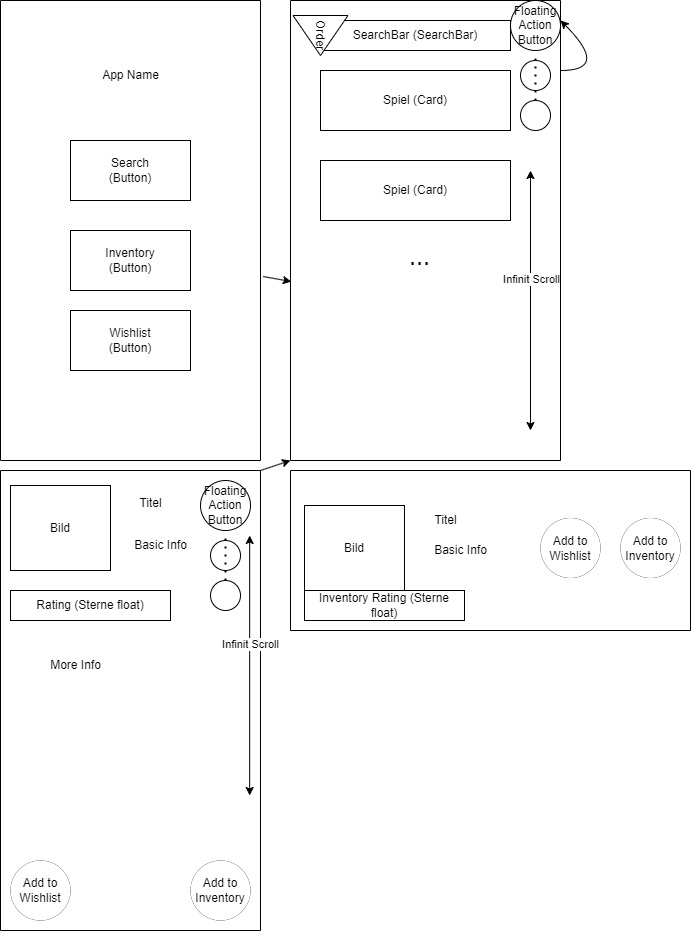
\includegraphics[width=0.6\textwidth]{graphics/konzept.jpeg}
    \caption{Erster Entwurf eines Konzeptes für die Benutzeroberfläche.}
    \label{fig:konzept}
\end{figure}

\section{HTML-Dokumentation}
\subsection{Einführung}
Diese HTML-Dokumentation bietet einen Überblick über die Architektur und die verschiedenen Seiten unseres Projekts,
welche mithilfe des Ionic Frameworks entwickelt wurde. Die Anwendung besteht aus einem intuitiven Design, welches auf die Präsentation von Spielen fokussiert
ist und verschiedene Funktionen wie Suche, Inventarverwaltung und Wunschliste bietet.
\subsection{Allgemeine Beobachtungen}
Unsere Anwendung nutzt das Ionic Framework und besteht aus einem Header- und einem Content-Bereich.
Ein „\ac{FAB}“ mit Navigationsoptionen befindet sich in der rechten oberen Ecke. Die Inhalte der Seiten werden mithilfe von Ion-Komponenten wie ion-card und ion-searchbar gestaltet.
\subsection{Details zu den Seiten}
\begin{enumerate}
    \item \texttt{Home.page.html} - Die Startseite präsentiert ein zufälliges Spiel des Tages mit einem minimalistischen Design und drei Buttons für die Suche, das Inventar und die Wunschliste.
    \item \texttt{Info.page.html} - Diese Detailseite zeigt Informationen zu einem einzelnen Spiel an, wie Name, Bild, Bewertung und Beschreibung. Es gibt auch Optionen zum Hinzufügen / Entfernen des Spiels aus der Wunschliste und dem Inventar.
    \item \texttt{Inventory.page.html} - Hier werden alle Spiele im Inventar des Benutzers aufgelistet, wobei ion-card-Elemente verwendet werden, um jedes Spiel mit Bild und Name anzuzeigen. Das Scrollen lädt weitere Spiele nach.
    \item \texttt{Search.page.html} - Diese Seite ermöglicht die Suche nach Spielen anhand von Keywords mit dynamischen Vorschlägen und einer Liste der gefundenen Spiele.
    \item \texttt{Wishlist.page.html} - Ähnlich als die "Inventory"-Seite listet diese Seite alle Spiele in der Wunschliste des Benutzers auf, wobei die Struktur und Funktionen identisch sind.
\end{enumerate}
\subsection{Besondere Merkmale}
Die Anwendung bietet dynamische Inhalte, da Spiele auf den Seiten „Inventory“, „Search“ und „Wishlist“ dynamisch aus dem Datenbestand geladen werden.
Infinite Scroll wird unterstützt, um nahtloses Laden weiterer Inhalte zu ermöglichen. Zudem passt sich die Anwendung mit responsive Design automatisch an verschiedene Bildschirmgrößen und Geräte an.
\section{SCSS-Dokumentation}
\subsection{Einführung}
Die SCSS-Dokumentation bietet einen umfassenden Überblick über das Design und die Gestaltungsentscheidungen für das vorliegende Projekt.
Dabei wird besonderen Wert auf eine elegante Farbpalette, klare Typografie und ein flexibles Layout gelegt, um ein professionelles und modernes Erscheinungsbild zu erzeugen.
\subsection{Allgemeine Designentscheidungen}
Für die Farbpalette wurde sich für dunkle und elegante Töne entschieden, die eine professionelle Atmosphäre schaffen sollen.
Akzentfarben wie Gelb und Hellblau bringen Leichtigkeit und Abwechslung ins Design, während eine harmonische Abstimmung der Farben für ein angenehmes Nutzererlebnis sorgt.
\newline
Für die Typografie wurde die gut lesbare Schriftart „Nyala“ gewählt und es wurden die Größen sowie der Zeilenabstand entsprechend für verschiedene Bildschirmgrößen angepasst.
\newline
Das Layout basiert auf Flexbox für Flexibilität und zentrierte Elemente sowie Media Queries zur Anpassung an verschiedene Bildschirmgrößen.
\subsection{Spezifische Designelemente}
Der Header präsentiert sich mit einem dunkelgrauen Hintergrund und weißem Text, um den Fokus auf den Inhalt zu lenken. Ähnlich minimalistisch ist auch der Content gestaltet, mit einem gut lesbaren Grau und Weiß.
\newline
Buttons heben sich durch einen dunkelgrauen Hintergrund und weißen Text ab, wobei unterschiedliche Farben je nach Funktion verwendet werden. Sie zeigen Interaktivität durch leichte Animationen beim Hover-Effekt.
\newline
Karten und Icons folgen ähnlichen Designrichtlinien, mit klaren Farben und gut sichtbaren Symbolen, die zur jeweiligen Funktion passen. Hier wurde auch besonders bei den Karten darauf geachtet, welche Informationen für den Nutzer relevant sind und welche Informationen erst bei genauerer Betrachtung des Spiels relevant sind, zu denen bspw. die Spieldauer gehört.
\newline
Der \ac{FAB} setzt auf Kontrast mit einem schwarzen Button und weißem Icon, um Aufmerksamkeit zu erregen.
\subsection{Begründung der Designentscheidungen}
Die Wahl der Farben und Formen dient nicht nur der Ästhetik, sondern auch der Nutzererfahrung wie z.B das große anzeigen des Spielbildes auf der Infopage für den Nutzer. Durch die Verwendung von dunklen Farben wird eine elegante und professionelle Atmosphäre geschaffen, während Akzentfarben wichtige Elemente hervorheben und für visuelle Abwechslung sorgen.
Die Schriftart und das Layout wurden mit Blick auf Lesbarkeit durch das Beispielsweiße anzeigen der wichtigsten Spiele Infos als Tabelle und Anpassungsfähigkeit entwickelt, um sicherzustellen, dass die App auf verschiedenen Geräten gut aussieht und einfach zu bedienen ist
Insgesamt wurde der SCSS-Code sorgfältig gestaltet, um ein konsistentes und ansprechendes Design zu gewährleisten, das den Anforderungen an eine moderne und nutzerfreundliche Anwendung gerecht wird.
\section{TypeScript-Dokumentation}
\subsection{Einführung}
Die TypeScript-Dokumentation bietet einen detaillierten Einblick in die Komponenten und Funktionalitäten des auf dem Angular-Framework basierenden Projekts. Es werden die Importe,
die Komponentendefinition und die Funktionalität der Hauptkomponente „app-home“ erläutert,
welche grundlegende Funktionen für die Startseite der Anwendung bereitstellt. Zusätzlich werden Erweiterungen und Beispielhinweise für eine bessere Verständlichkeit des Codes bereitgestellt.
\subsection{Komponenten und Importe}
Die Importe umfassen verschiedene Module wie \texttt{@angular/core} und \texttt{@angular/router},
die für die Komponentenerstellung und die Navigation innerhalb der Anwendung benötigt werden. Zusätzlich werden Services und Modelle importiert, um Daten abzurufen und zu strukturieren.
\subsection{Komponentendefinition}
Die „app-home“ Komponente wird durch den Selektor „app-home“ referenziert und besteht aus einer Template-Datei und einem Stylesheet, die das Aussehen und Verhalten der Komponente definieren.
\subsection{Funktionalität}
Im Konstruktor werden erforderliche Services und Router für die Navigation injiziert. Die \texttt{ngOnInit()}-Methode wird verwendet, um bei jeder Navigation ein zufälliges Top-Spiel abzurufen und die Daten zu aktualisieren.
\subsection{Zusätzliche Hinweise}
Der Code verwendet das \texttt{Randomgame}-Interface, um die Struktur der abgerufenen Spieldaten festzulegen. Die Navigation erfolgt über relative Pfade für eine konsistente und interne Routenführung.
\subsection{Erweiterungen}
Es werden Funktionen wie \texttt{goToSearch()}, \texttt{goToInventory()} und \texttt{goToWishlist()} beschrieben, die zur Navigation zu bestimmten Seiten innerhalb der App dienen. Jede Funktion wird erklärt und ihr Zweck sowie das Ziel der Navigation angegeben.
\subsection{Beispiel}
\texttt{goToSearch()}: Navigiert zur „/searchpage“-Route, um die Suche nach Spielen zu ermöglichen.
\section{Beschreibung der erstellten Mockups}
In diesem Kapitel wird ein Blick auf die Entwicklung der App vom anfänglichen Mockup bis zum fertigen Endprodukt geworfen. Es werden die wichtigsten Änderungen und Anpassungen erläutert,
die während des Entwicklungsprozesses vorgenommen wurden, während zeitgleich hervorgehoben wird, welche Elemente des Mockups unverändert geblieben sind.
\subsection{Änderungen und Anpassungen}
\begin{enumerate}
    \item \textbf{Detaillierte Spielinformationen:} Die Detailseiten der Spiele sind um zusätzliche Informationen erweitert worden. Videos, Bildschirmfotos, Rezensionen und Spielerbewertungen sind nun ebenfalls einsehbar (siehe Abb. \ref{fig:detailseite}).
    \item \textbf{Verbessertes Design:} Das Design der App ist im Laufe des Entwicklungsprozesses kontinuierlich optimiert worden. Insbesondere die Gestaltung der Benutzeroberfläche und die Farbgebung sind fortlaufenden Verbesserungen unterzogen worden.
\end{enumerate}
\begin{figure}[H]
    \centering
    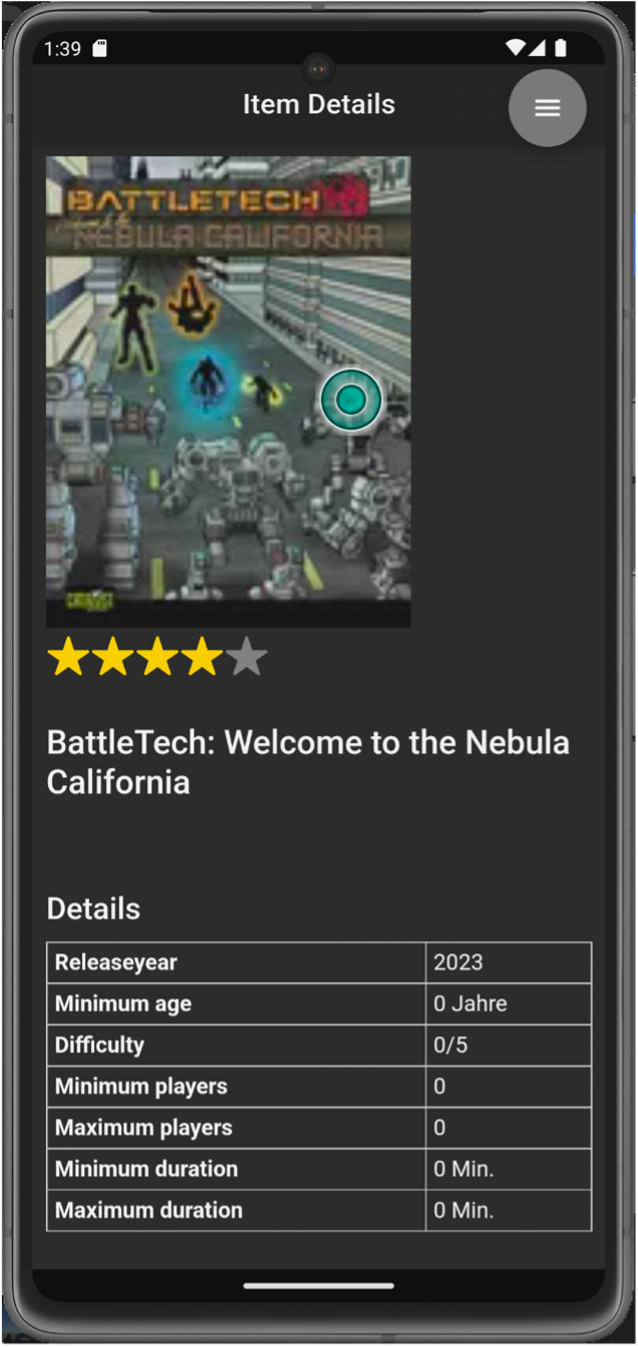
\includegraphics[width=0.4\textwidth]{graphics/infopage.png}
    \caption{Optimierte Detailseite eines Spiels.}
    \label{fig:detailseite}
\end{figure}
\subsection{Unveränderte Elemente}
\begin{enumerate}
    \item \textbf{Grundlegende Struktur:} Die zugrundeliegende Struktur, zu welcher die Hauptnavigation und die Anordnung der Hauptkomponenten gehören, ist im Wesentlichen unverändert geblieben.
    \item \textbf{Kernfunktionen:} Die Kernfunktionen der App, wie die Suche nach Spielen, die Anzeige detaillierter Informationen zu Spielen sowie die Verwaltung von Spielen in Wunschliste und Inventar, haben auch nach Erstellung des Mockups noch Bestand.
\end{enumerate}
\subsection{Fazit}
Die Entwicklung der App vom Mockup bis zum Endprodukt kann als iterativer Prozess angesehen werden, welcher
von ständigen Verbesserungen und Anpassungen geprägt war. Hierbei konnten sich die Kernfunktionen der App
als stabil erweisen, während für Design und Benutzerobefläche kontinuierliche Optimierungspotentiale bestanden (siehe Fig. \ref{fig:optimierung}).
In dem Zuge sind auch neue Funktionenen dem Projekt hinzugefügt worden, auch wenn diese nicht im ursprünglichen
Mockup enthalten waren. Ziel war eine kontinuierliche Verbesserung der Benutzererfahrung und Erweiterung des Funktionsumfangs.
\begin{figure}[H]
    \centering
    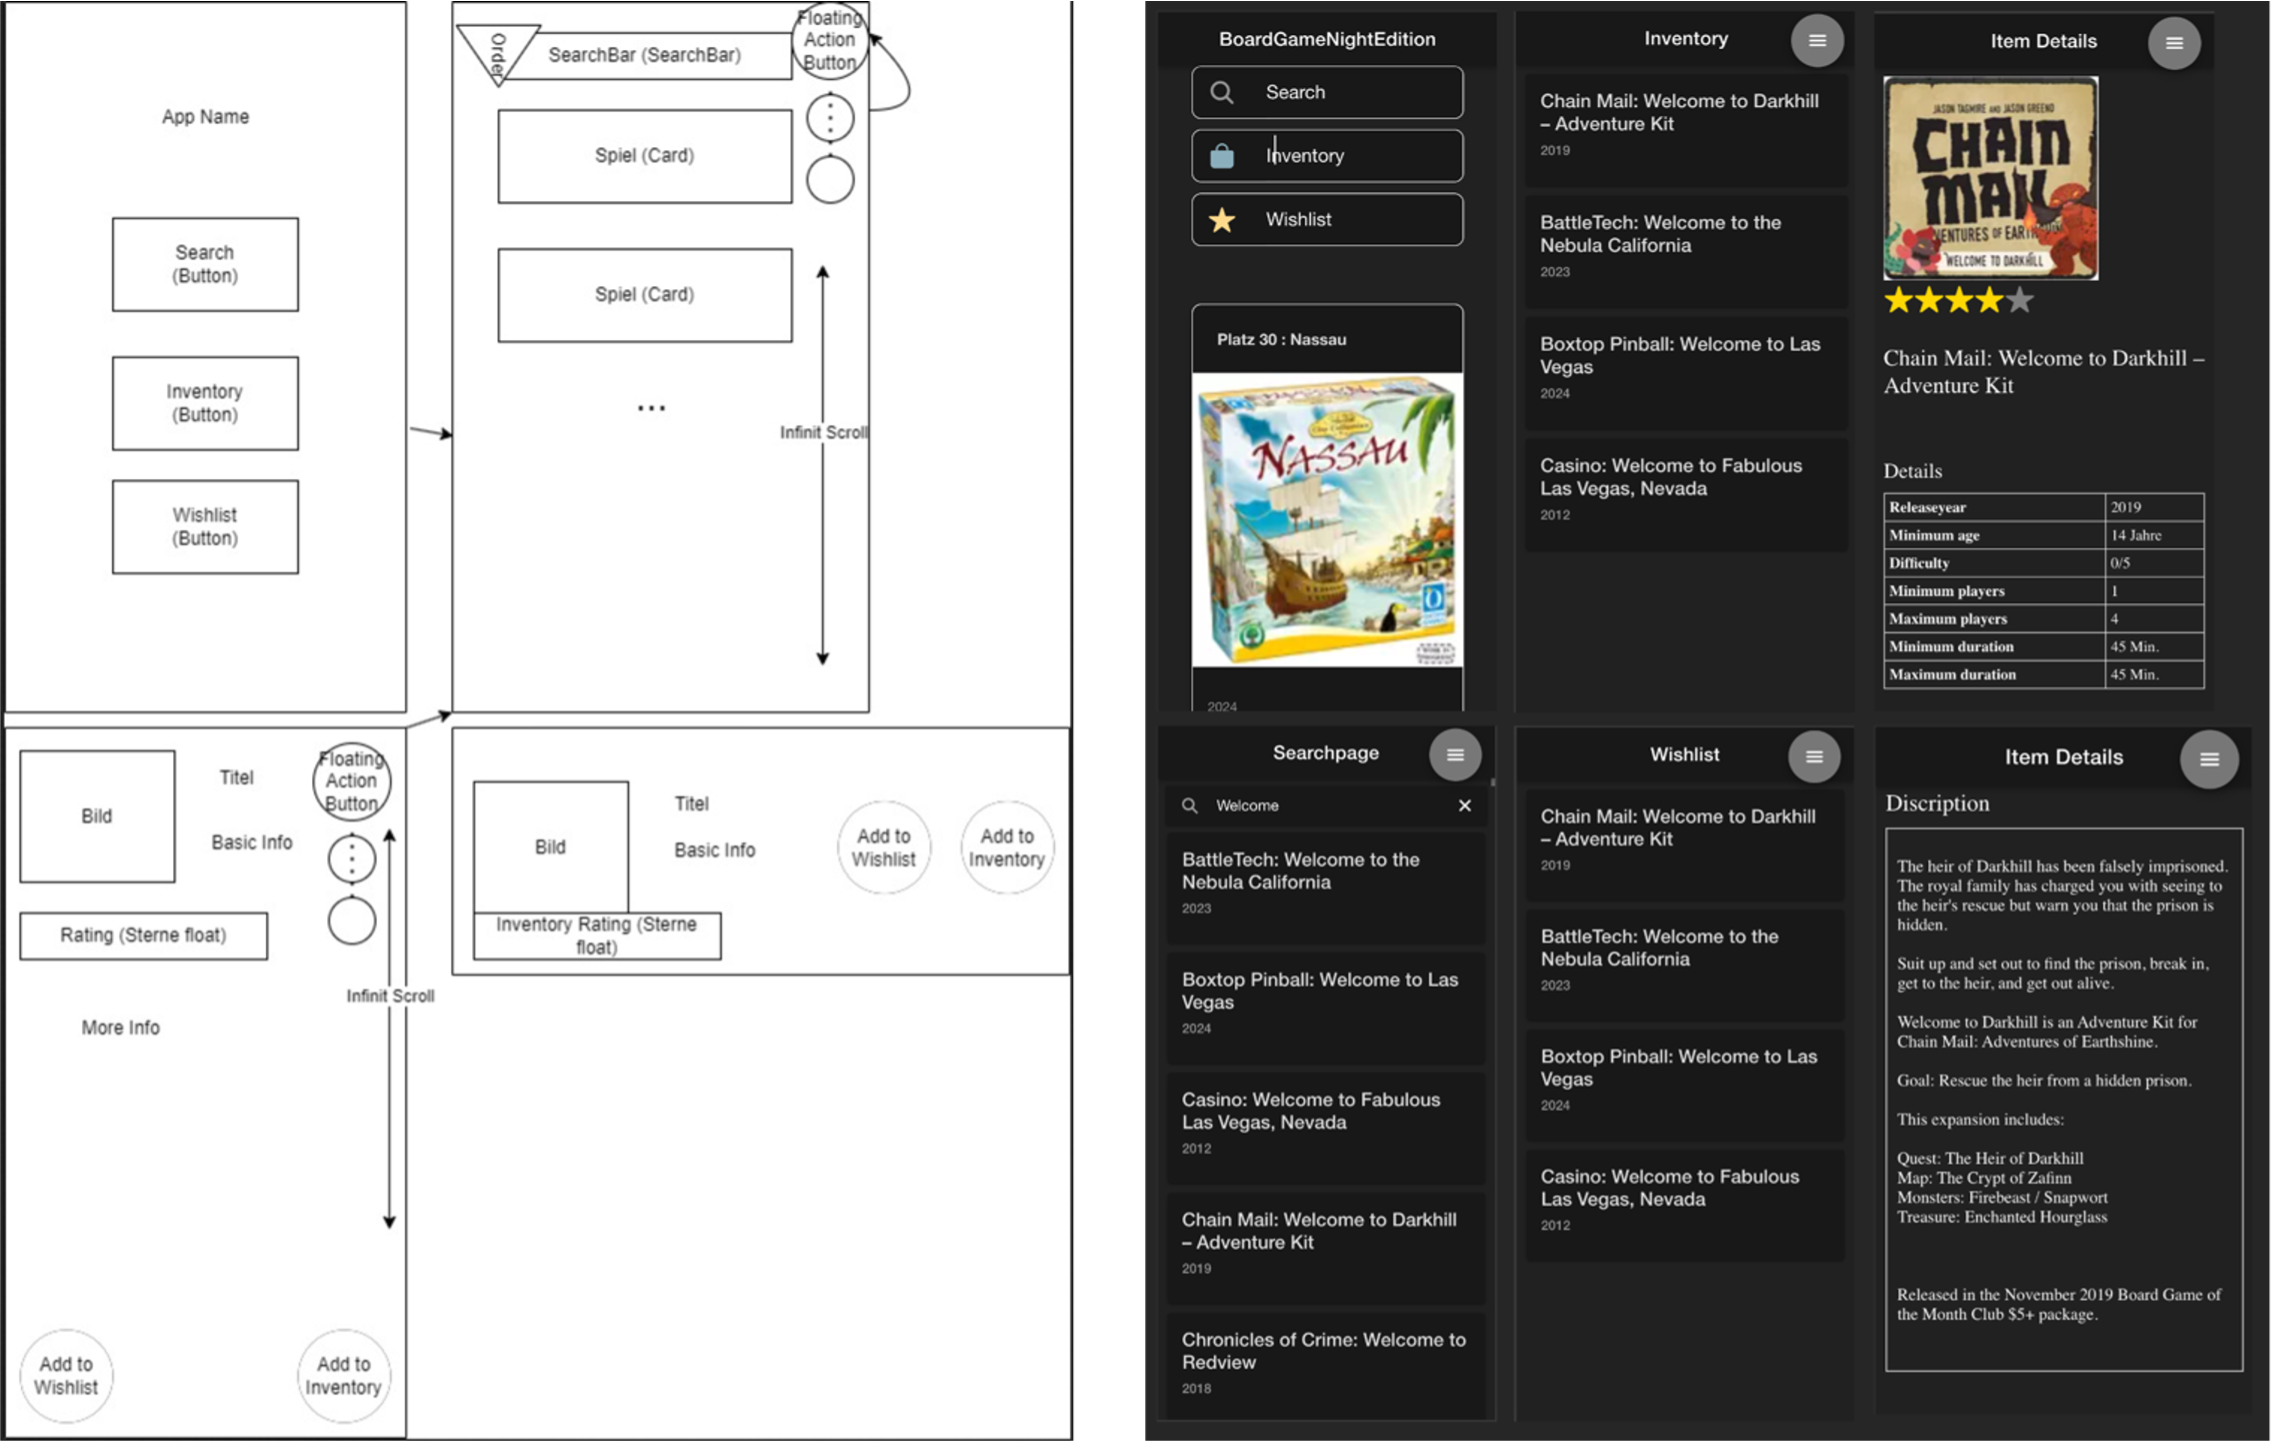
\includegraphics[width=1\textwidth]{graphics/mockup_vergleich.png}
    \caption{Mockup-Vergleich (alt vs. neu).}
    \label{fig:optimierung}
\end{figure}
\chapter{Technische Umsetzung}
\section{Beschreibung der App}
\subsection{Funktionen der jeweiligen Seiten}
\subsubsection{Homepage}
Die Homepage der App zeigt ein zufälliges und derzeit besonders beliebtes Spiel an, welches von der BoardGameGeek \ac{API} bezogen wird.
Die Generierung erfolgt automatisch und bei jedem Aufruf der Seite neu. Daher wird dieser Fähigkeit in der \texttt{ngOnInit()}-Funktion auf der Homepage aufgerufen.
Darüber hinaus dient die Homepage primär als Ausgangspunkt für die Navigation zu den anderen Seiten (siehe Tab. \ref{tab:homepage}).
\begin{table}[H]
    \centering
    \begin{tabular}{|c|c|}
        \hline
        \textbf{Funktion} & \textbf{Beschreibung} \\
        \hline
        \texttt{goToSearch()} & Navigiere zur Suchleiste. \\
        \texttt{goToWishlist()} & Navigiere zur Wunschliste. \\
        \texttt{goToInventory()} & Navigiere zum Inventar. \\
        \texttt{openGameDetails()} & Navigiere zur Infopage des zufälligen Spiels. \\
        \hline
    \end{tabular}
    \caption{Funktionen der Homepage.}
    \label{tab:homepage}
\end{table}

\subsubsection{Searchpage}
\subsubsection{Infopage}
\subsection{Genutzte Interfaces und Modelle}
In der Welt der Softwareentwicklung ist es entscheidend, dass Daten, die zwischen verschiedenen
Systemen ausgetauscht werden, klar definierte Strukturen haben. TypeScript-Interfaces sind hierbei
äußerst nützlich, insbesondere wenn es um die Interaktion mit APIs geht.
Das Boardgame Interface beschreibt alle wesentlichen Informationen eines Brettspiels, die über die
BGG-API abgerufen werden und in einer MongoDB gespeichert werden. Dazu gehören Details wie der
eindeutige Identifikator des Spiels, das Veröffentlichungsjahr, die Spieleranzahl, die Spieldauer, das
empfohlene Alter, eine Beschreibung und ein Vorschaubild. Dieses Interface stellt sicher, dass die von
der API gelieferten Daten vollständig und in einer korrekten Form sind, die direkt in der Datenbank
gespeichert werden kann (so dass auch Falls kein Bild in der Api Verfügbar ist dies abgespeichert
wird).
Das Game Interface hingegen ist eine reduzierte Version des Boardgame Interfaces. Es kann in
Situationen eingesetzt werden, in denen nicht alle Informationen eines Brettspiels benötigt werden,
wie zum Beispiel in einer Übersichtsliste von Spielen. Durch das Weglassen von Details wie Spielzeit
oder Altersangabe wird die übertragene Datenmenge verringert, was die Effizienz verbessern und die
Ladezeiten verkürzen kann.
Das Randomgame Interface ist spezialisiert auf die Darstellung eines zufällig ausgewählten Spiels aus
den Top 50 der am besten bewerteten Brettspiele. Neben der Standardinformation wie Identifikator,
Name, Veröffentlichungsjahr und einem Bild des Spiels, speichert dieses Interface zusätzlich den Rang
des Spiels, also seine Position in der Rangliste. Diese Information ist besonders wertvoll, um auf einen
Blick die Beliebtheit eines Spiels einschätzen zu können, diese wird basierend auf ihrer Position in der
Top 50 eingelesen.
Diese Interfaces sind essenzielle Bausteine für die zuverlässige Datenarchitektur. Sie sorgen nicht nur
für eine korrekte Typisierung und eine klare Vertragsgestaltung zwischen dem Backend (der API) und
dem Frontend, sondern tragen auch dazu bei, den Datenfluss übersichtlich und wartbar zu halten. So
kann die Software sich an verändernde Anforderungen anpassen, ohne dass es zu einem
Durcheinander in der Datenstruktur kommt.

\subsubsection{Boardgame}
Das \texttt{Boardgame} Interface repräsentiert die Struktur zur Speicherung von Informationen über ein
Brettspiel. Die Eigenschaften sind wie folgt:
\begin{table}[H]
    \centering
    \begin{tabular}{|c|c|c|}
        \hline
        \textbf{Eigenschaft} & \textbf{Typ} & \textbf{Beschreibung} \\
        \hline
        \texttt{objectId} & \texttt{string} & Dient der eindeutigen Identifikation eines Spiels. \\
        \texttt{yearPublished} & \texttt{string} & Das Jahr, in dem das Spiel veröffentlicht wurde. \\
        \texttt{minPlayers} & \texttt{string} & Die minimal erforderliche Anzahl an Spielern. \\
        \texttt{maxPlayers} & \texttt{string} & Die maximal mögliche Anzahl an Spielern. \\
        \texttt{playingTime} & \texttt{string} & Die durchschnittliche Spieldauer. \\
        \texttt{minPlayTime} & \texttt{string} & Die minimal mögliche Spieldauer. \\
        \texttt{maxPlayTime} & \texttt{string} & Die maximal mögliche Spieldauer. \\
        \texttt{age} & \texttt{string} & Die empfohlene Altersangabe. \\
        \texttt{description} & \texttt{string} & Eine Beschreibung des Spiels. \\
        \texttt{name} & \texttt{string[]} & Eine Liste von Namen, unter denen das Spiel bekannt ist. \\
        \texttt{publisher} & \texttt{string[]} & Eine Liste von Verlagen, die das Spiel veröffentlicht haben. \\
        \texttt{averageWeight} & \texttt{string} & Die durchschnittliche Komplexität des Spiels. \\
        \texttt{averageRating} & \texttt{string} & Die durchschnittliche Bewertung des Spiels. \\
        \texttt{thumbnail} & \texttt{string} & Ein Link zu einem Vorschaubild des Spiels. \\
        \texttt{usersRated} & \texttt{string} & Die Anzahl der Benutzer, die das Spiel bewertet haben. \\
        \hline
    \end{tabular}
    \caption{Eigenschaften des \texttt{Boardgame} Interfaces.}
    \label{tab:boardgame}
\end{table}

\subsubsection{Game}
Das \texttt{Game} Interface repräsentiert eine reduzierte Version des \texttt{Boardgame} Interfaces. Es
wird verwendet, um die Datenmenge zu verringern, wenn nicht alle Informationen eines Spiels
benötigt werden. Die Eigenschaften sind hierbei wie folgt:
\begin{table}[H]
    \centering
    \begin{tabular}{|c|c|c|}
        \hline
        \textbf{Eigenschaft} & \textbf{Typ} & \textbf{Beschreibung} \\
        \hline
        \texttt{objectId} & \texttt{string} & Dient der eindeutigen Identifikation eines Spiels. \\
        \texttt{name} & \texttt{string} & Gibt den Namen des Spiels an. \\
        \texttt{yearPublished} & \texttt{string} & Das Jahr, in dem das Spiel veröffentlicht wurde. \\
        \texttt{thumbnail} & \texttt{string} & Ein Link zu einem Vorschaubild des Spiels. \\
        \hline
    \end{tabular}
    \caption{Eigenschaften des \texttt{Game} Interfaces.}
    \label{tab:game}
\end{table}
\textbf{Hinweis:} Es gibt zwei Versionen des \texttt{Game} Interfaces, eine mit der Eigenschaft „thumbnail“ und eine
ohne. Es ist wichtig sicherzustellen, dass die richtige Version verwendet wird, um der erforderlichen
Datenstruktur für die Anwendung zu entsprechen.

\subsubsection{Randomtopgame}
Das \texttt{Randomtopgame} Interface repräsentiert die Struktur zur Speicherung von Informationen über ein
zufällig ausgewähltes Spiel aus den Top 50 der am besten bewerteten Brettspiele. Hierfür werden folgende
Eigenschaften definiert:
\begin{table}[H]
    \centering
    \begin{tabular}{|c|c|c|}
        \hline
        \textbf{Eigenschaft} & \textbf{Typ} & \textbf{Beschreibung} \\
        \hline
        \texttt{id} & \texttt{string} & Dient der eindeutigen Identifikation eines Spiels. \\
        \texttt{name} & \texttt{string} & Der Name des Spiels. \\
        \texttt{yearPublished} & \texttt{string} & Das Jahr, in dem das Spiel veröffentlicht wurde. \\
        \texttt{thumbnail} & \texttt{string} & Ein Link zu einem Vorschaubild des Spiels. \\
        \texttt{rank} & \texttt{string} & Die Position des Spiels in der Rangliste. \\
        \hline
    \end{tabular}
    \caption{Eigenschaften des \texttt{Randomtopgame} Interfaces.}
    \label{tab:randomtopgame}
\end{table}
\section{Beschreibung der verwendeten Services}


\section{Beschreibung der verwendeten APIs}
\subsection{BoardGameGeek XML API }

Die BoardGameGeek XML API bietet eine Schnittstelle zum Zugriff auf eine Vielzahl von Informationen rund um Brettspiele,
die auf BoardGameGeek.com, einer umfangreichen Datenbank und Community für Brettspiel-Enthusiasten,
verfügbar sind. Diese API ermöglicht es Entwicklern druch verschiedene Endpoints auf Spielinformationen,
Benutzerkollektionen und Forendiskussionen zuzugreifen. Dabei zu beachten ist, dass die API die Antwort als XML-Format weitergibt. 
Da häufig mit JSON gearbeitet wird ist eine mögliche Umformung der Daten sinnvoll.

\large Suchfunktion

Eine der drei benutzten Endpunkte ist die `/xmlapi/search`-Funktion bei der Nutzer als Input einem spezifischen Suchterm eingeben.
Als Ergebnis enthält man eine Liste an Brettspielen in XML Format, deren Namen oder Alias im Suchbegriff enthalten war.
Die Suchfunktion Antwort enthält folgende Informationen:
\begin{itemize}
    \item {objectId des Brettspiels}
    \item {Name des Brettspiels}
    \item {Erscheinungsjahr des Brettspiels}
\end{itemize}

Die reale Ausgabe für den fiktiven Suchterm ``Frika'' würde somit folgendes zurückgeben: 
\begin{figure}[h]
    \centering
    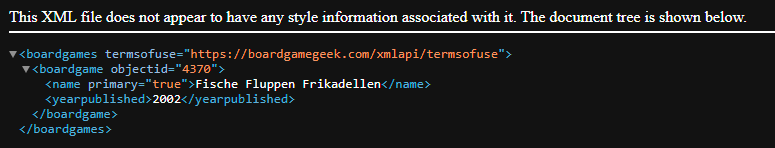
\includegraphics[width=1\textwidth]{graphics/Search_API.png}
    \caption{Ergebnis der `/xmlapi/search`-Funktion bei Suchterm Frika}
    \label{fig:Search_API}
\end{figure}

 \large Detaillierte Spielinformationen

Der zweite Endpunkt ist die `/xmlapi/boardgame/<gameid>`-Funktion und dient dazu,
detaillierte Informationen zu einem Brettspiel zu erhalten. Nutzer könnten hier noch einige weitere Parameter mitgeben um spezifische Informationen zu erhalten, jedoch ist dies in unserem Projekt nicht notwendig, da die Ergebnisse schon detailliert genug sind.
Die gameId ist hierbei der Input, ist gleichzusetzen mit der objectId und kann aus des oben erhaltenen Ergebnisses der Suchfunktion entnommen werden.
Die detaillierten Spielinformationen enthalten folgende Informationen:
% Reduzieren des Abstands zwischen den Punkten
\begingroup
\setlength{\itemsep}{-1pt} % Setzt den Abstand zwischen den Punkten auf 0pt
\setlength{\parskip}{-1pt} % Optional: Reduziert den Abstand zwischen Absätzen
\begin{itemize}
    \item objectId: String
    \item yearPublished: String
    \item minPlayers: String
    \item maxPlayers: String
    \item playingTime: String
    \item minPlayTime: String
    \item maxPlayTime: String
    \item age: String
    \item description: String
    \item name: Array (String)
    \item publisher: Array (String)
    \item averageWeight: String
    \item averageRating: String
    \item thumbnail: String (URL to thumbnail image)
    \item usersRated: String
\end{itemize}
\endgroup

Es ist zu erkennen, dass der Name und der Publisher Arrays sind. Dies lässt sich darauf zurückführen, dass es mehrere Namen für dasselbe Spiel gibt (teilweise auch in anderen Sprachen) und mehrere Entwicklet beteiligt sein können.

\large Game of the Day

Der dritte Endpunkt im Bunde ist die `xmlapi2/hotoverall`-Funktion. Sie gibt die top 50 Spiele mit besonders guter Bewertung und Beliebtheit zurück.
Dabei werden genau fünf unterschiedliche Informationen aufgeführt:
\setlength{\itemsep}{-1pt}
\setlength{\parskip}{-1pt}
\begin{itemize}
    \item id: String (objectId von vorher earlier)
    \item rank: String (Ranking Position der Top 50 Spiele)
    \item thumbnail: String (URL to thumbnail image)
    \item name:  String        
    \item yearpublished 
\end{itemize}

Im Anschluss kann ebenfalls mit der ObjectId eine Anfrage für detaillierte Informationen gestartet werden, die dann auf der Infopage angezeigt werden. 

\subsection{MongoDB API}

In diesem Teil wird nur der externe Aufruf auf den selbsterstellten MongoDB API-Endpunkt behandelt. 
Der Interne Aufbau der MongoDB wird in der Beschreibung der App aufgeführt. Es gibt insgesamt drei Zugriffsmethoden für jede Collection auf die MongoDB: 
searchGamesWishlist(), searchGamesInventory(), addToWishlist(gameData), addToInventory(gameData), removeFromWishlist(objectId), removeFromInventory(objectId)\bigskip


Die Get Methode bezieht sich af den HTTP Endpoint ``http://localhost:8999/wishlisht'' oder beziehungsweise ``\ldots/inventory'' und liefert eine Liste aus JSON-Elementen zurück.
Für das hinzufügen von Brettspielen wird die HTTPClient Methode POST benutzt und die gameData übergeben, wobei Gamedata ein Objekt des Modells Boardgame.ts ist. 

\begin{center}
    \begin{lstlisting}[caption={Löschaufruf der MongoDB API}, label=lst:jscode]
    this.http.delete(`${this.inventoryUrl}/${objectId}`)
\end{lstlisting}
\end{center}


\subsection{Verwendung der APIs im Projekt selbst}

Die Definition der Methoden zum aufrufen der API-Endpunkte ist in dem   File ``board-game.service.ts'' des ``services''-Ordner zu finden.
Dazu wird das HTTPClient Modul importiert und es wird ein htttp.get Aufruf mit den jeweiligen Parametern durchgeführt. Da das Ergebnis in Form einer XML-Datei vorliegt und es vorteilhafter ist mit einem JSON-Format zu arbeiten wird zu Beginn eine Transfarmation des Formats in die JSON Form durchgeführt.
Dies geschieht konkret durch das importierte Modul ``xml2json''. \bigskip 

Die daraufhin vorliegende JSON kann nun dem Modell game.ts, boardgame.ts oder randomtopgame.ts zugewiesen werden. Also eine initialisierung einer Liste von Objekte dieser Modelle basierend auf dem spezifischen API-Aufruf.
Im folgenden wird dann Array als return Element der Funktion definiert. Dies ermöglicht es erstmalig ein subscribe auf die Funktion zu legen und auf der benötigten Page anzuzeigen. \bigskip 

Die konkrete Verwendung der APIs auf den folgenden Pages ist wiefolgt:

\begin{itemize}
    \setlength{\itemsep}{-1pt}
    \setlength{\parskip}{-1pt}
    \item Homepage
        \begin{itemize}
        \item Game of the Day mit `xmlapi2/hotoverall`-Funktion
        \end{itemize}
    \item Searchpage
        \begin{itemize}
        \item Suchfunktion mit `/xmlapi/search`-Funktion
        \end{itemize}
    \item Inventory, Wishlist
        \begin{itemize}
        \item MongoDB mit `http://localhost:8999/inventory`-Funktion oder `.../wishlist` 
        \end{itemize}
    \item Infopage
    \begin{itemize}
    \item Detaillierte Spielinformationen mit `/xmlapi/boardgame/<gameid>`-Funktion 
    \end{itemize}

\end{itemize}

\section{Anleitung zum Starten der Applikation}

\chapter{Aufteilung des Projektes}

\chapter{Zusammenfassung und Ausblick}




\chapter*{Anhang}
\addcontentsline{toc}{chapter}{Anhang}
\section*{Anhangverzeichnis}
\vspace{-8em}

% vor \listofanhang müssen Einrückungen angepasst werden
\abstaendeanhangverzeichnis

\listofanhang
\clearpage
\spezialkopfzeile{Anhang} % damit in der Kopfzeile das Wort "Anhang" angezeigt wird

\anhang{Anhang 1}\label{anhang:kap1}
% \anhangteil{Unterkapitel 1}\label{anhang:ukap1}
\anhang{Anhang 2}\label{anhang:kap2}
\anhang{Anhang 3}\label{anhang:kap3}


\lstset{language=TeX, % hervorzuhebende Keywords definieren
  morekeywords={anhang, anhangteil}
}

% \blinddocument
% \chapter{Beispiele für Abbildungen und Tabellen}\label{chapter:abbildungenTabellen}

Hier finden Sie Beispiele für Abbildungen, Tabellen, Formelsatz und  Source Code.

\section{Abbildungen}
In diesem Abschnitt gibt die Abbildungen~\ref{abb:Logo2cmHoch} und~\ref{abb:Logo2cmBreit}, die beide das Logo der DHBW zeigen.

\begin{figure}[htb]
\centering

\includegraphics[height=2cm]{graphics/dhbw.png}
\caption[DHBW-Logo 2cm hoch]{DHBW-Logo 2cm hoch.\footnotemark}
\label{abb:Logo2cmHoch}
\end{figure}
\footnotetext{Mit Änderungen entnommen aus: \cite{OhneAutorenOhneJahr}}

\lstset{language=TeX, % hervorzuhebende Keywords definieren
  morekeywords={footnotetext,footnotemark,footcite,caption}
}

\emph{Spezialfall:} Sofern \emph{innerhalb} der Bezeichnung einer Abbildung eine Fußnote angegeben oder eine Quelle referenziert werden soll, geschieht dies nicht per \lstinline|\footnote| oder \lstinline
|\footcite|. Vielmehr sind die Befehle \lstinline|\footnotemark| und \lstinline|\footnotetext| zu verwenden und außerdem das optionale Argument für \lstinline|\caption| anzugeben (vgl.\ Source Code).

\begin{figure}[htb]
\centering

\includegraphics[width=2cm]{graphics/dhbw.png}
\caption[DHBW-Logo 2cm breit.]{DHBW-Logo 2cm breit. (Quelle: DHBW\footnotemark)}
\label{abb:Logo2cmBreit}
\end{figure}
\footnotetext{\url{www.dhbw.de}}



\section{Tabellen}

In diesem Abschnitt gibt es zwei Beispiel-Tabellen, nämlich auf Seite~\pageref{tab:BeispielTabelleKlein} und auf Seite~\pageref{tab:BeispielTabelleGroesser}.

\begin{table}[htb]
\centering
\begin{tabular}{lcr}
links & Mitte & rechts \\
\hline
Muster & Muster & Muster \\
\end{tabular}
\caption{Kleine Beispiel-Tabelle.}
\label{tab:BeispielTabelleKlein}
\end{table}

\begin{table}[htb]
\centering
\begin{tabular}{|l|l|c|l|r||l}
    \textbf{Spalte 1} & \textbf{Spalte 2} & \textbf{Spalte 3} & \textbf{Spalte 4} & \textbf{Spalte 5} & \textbf{Spalte 6} \\
    \hline
    a        & b          & c                & d        & e        & f        \\
    Test     & Test, Test & Test, Test, Test & ~        & ~        & ~        \\
    1        & 2          & 3                & 4        & 5        & 6        \\
\end{tabular}
\caption{Größere Beispiel-Tabelle.}
\label{tab:BeispielTabelleGroesser}
\end{table}

\section{Etwas Mathematik}

Eine abgesetzte Formel:
\[
  \int_a^b x^2 \: \mathrm{d} x = \frac{1}{3} (b^3 - a^3)
\]

Es ist $a^2+b^2 = c^2$ eine Formel im Text.

\section{Source Code}

Source Code-Blöcke können auf folgende Arten eingefügt werden:

\lstset{language=Java}

Direkt im \LaTeX-Source Code:
\begin{lstlisting}
if(1 > 0) {
  System.out.println("OK"); 
} else {
  System.out.println("merkwuerdig");
}
\end{lstlisting}

oder eingefügt aus einer externen Datei.
\lstinputlisting{includes/HelloWorld.java}

% \anhang{Release Notes}
\anhangteil{Änderungen in Version 1.1}\label{anhang:ReleaseNotes11}
In Version 1.1 sind einige Rückmeldungen, die nach der Einführungsvorlesung am 6.2.2015 oder nach Veröffentlichung der Vorlage in Moodle eingegangen sind, berücksichtigt worden. Korrekturen sind mit \enquote{(Fix)} gekennzeichnet. 

\begin{itemize}
\item \verb|latex-vorlage.tex|
\begin{itemize}
\item (Fix) Abkürzungsverzeichnis wird vor Abbildungsverzeichnis platziert
\item (Fix) Abbildungs- und Tabellenverzeichnis in Inhaltsverzeichnis aufgenommen
\item (Fix) Quellenverzeichnis wird nun ohne Kapitelnummer dargestellt

\item eingebundene Dateien in Unterverzeichnissen \verb|includes| bzw.\ \verb|graphics|
\item Beispiel-Anhang (Datei \verb|anhang.tex|) mit Erklärungen wurde eingebunden 
\end{itemize}

\item \verb|_dhbw_praeambel.tex|
\begin{itemize}
\item (Fix) das Paket hyperref wird nach biblatex eingebunden, um ein Problem mit der Verlinkung der Fußnoten im PDF zu beheben
\item (Fix) Fußnoten  gemäß der Richtlinien fortlaufend nummeriert und nicht pro Kapitel
\item Einstellungen hinzugefügt, um Anhangsverzeichnis zu ermöglichen
\item bessere Kompatibilität zwischen KOMA-Script (scrreprt) und anderen Paketen mittels scrhack
\end{itemize}

\item \verb|_dhbw_biblatex-config.tex|
\begin{itemize}
\item (Fix) keine Abschnittsnummern für einzelne Verzeichnisse im Quellenverzeichnis
\end{itemize}

\item \verb|abbildungen_und_tabellen.tex|
\begin{itemize}
\item Erklärung, wie eine Fußnote/ein Zitat bei einer Abbildung zu erstellen ist
\end{itemize}

\item \verb|abkuerzungen.tex|
\begin{itemize}
\item Abkürzungsverzeichnis wird im Inhaltsverzeichnis aufgeführt
\end{itemize}

\item \verb|abstract.tex|, \verb|anhang.tex|, \verb|einleitung.tex| 
\begin{itemize}
\item Erklärungen im Text ergänzt
\end{itemize}

\item \verb|deckblatt.tex|
\begin{itemize}
\item Meta-Daten (Autor, Titel) für die generierte PDF-Datei lassen sich nun festlegen
\end{itemize}

\end{itemize}


\anhangteil{Änderungen in Version 1.2}\label{anhang:ReleaseNotes12}
Über das Forum in Moodle sind einige Rückmeldungen eingegangen -- vielen Dank an alle, die dazu beigetragen haben. In der Version 1.2 wurden folgende Änderungen vorgenommen, wobei Korrekturen wieder mit \enquote{(Fix)} gekennzeichnet sind: 

\begin{itemize}
\item \verb|latex-vorlage.tex| (Hauptdokument)
\begin{itemize}
\item (Fix) Zeile 19: Seitenzahlen zu Beginn mit römischen \emph{Groß}buchstaben nummeriert
\end{itemize}

\item \verb|_dhbw_praeambel.tex|
\begin{itemize}
\item Zeile 39/40: Unterstützung für \enquote{ebenda} 
\item Zeile 46--68: zweite Gliederungsebene für Anhänge ermöglicht
\item (Fix) Zeile 70--73: Abbildungen und Tabellen: Zähler fortlaufend, kein Rücksetzen zu Kapitelbeginn (Paket \verb|chngcntr| anstelle von Paket \verb|remreset|)
\end{itemize}

\item \verb|_dhbw_biblatex-config.tex|
\begin{itemize}
\item (Fix) bei Quellen mit Herausgeber, aber ohne Autor wird der Name des Herausgebers im Verzeichnis fett gedruckt
\item Unterstützung für \enquote{ebenda} 
\end{itemize}

\item \verb|abkuerzungen.tex|
\begin{itemize}
\item Bemerkungen zur fortgeschrittenen Nutzung des \verb|acronym|-Pakets eingefügt 
\end{itemize}

\item \verb|einleitung.tex|
\begin{itemize}
\item Abschnitt 1.3 zu Einstellungen ergänzt
\item Abschnitt 1.5 zu Fehlerbehebungen eingefügt 
\end{itemize}

\item \verb|text-mit-zitaten.tex|
\begin{itemize}
\item Abschnitt 3.1 eingefügt, Erläuterungen zum Zitieren mit \enquote{vgl.} und \enquote{ebenda}. 
\item Abschnitt 3.2: Beispiele ergänzt
\item Hinweis zu Jahreszahlen bei Online-Quellen
\end{itemize}

\item \verb|anhang.tex|
\begin{itemize}
\item Erläuterungen zur zweiten Gliederungsebene
\end{itemize}

\item \verb|literatur-datenbank.bib|
\begin{itemize}
\item weitere Beispiele für Quellen
\end{itemize}

\end{itemize}

\anhangteil{Änderungen in Version 1.3}\label{anhang:ReleaseNotes13}
Durch die ab 1/2016 geltenden Änderungen der Zitierrichtlinien des Studiengangs waren einige kleinere Anpassungen der Vorlage erforderlich, die nachfolgend beschrieben sind. Bei dieser Gelegenheit ebenfalls erfolgte Korrekturen sind wieder mit \enquote{(Fix)} gekennzeichnet:

\begin{itemize}
\item \verb|latex-vorlage.tex| (Hauptdokument)
\begin{itemize}
\item Hinweis auf Option doppelseitiger Druck entfernt
\item Schriftgröße der Kapitelüberschriften verkleinert
\item (Fix) Kopf- und Fußzeilen werden nun korrekt angezeigt für erste Seite eines Kapitels und auch  Quellenverzeichnisse
\end{itemize}

\item \verb|_dhbw_praeambel.tex|
\begin{itemize}
\item Angabe des unteren Rands für Seitenzahl, da diese nun unten rechts steht
\item Unterstützung für \enquote{ebenda} entfernt
\item (Fix) Präfixe wie \enquote{von} im Namen eines Autors werden berücksichtigt
\item Anpassung der Abstände bei Kapitelüberschriften
\item Kopf- und Fußzeile für Verzeichnisse nun in \verb|_dhbw_kopfzeilen.tex| definiert 
\end{itemize}


\item \verb|deckblatt.tex|
\begin{itemize}
\item Schriftgröße des Titels vergrößert
\item Befehl \verb|\typMeinerArbeit| eingeführt, um Typ auszuwählen
\item Festlegung des Themas (für ehrenwörtliche Erklärung) mit Befehl \verb|\themaMeinerArbeit|
\item Darstellung der Angabe des Betreuers in der Ausbildungsstätte angepasst
\item Formulierung des Sperrvermerks angepasst  
\end{itemize}

\item \verb|_dhbw_erklaerung.tex|
\begin{itemize}
\item Formulierung angepasst an geänderte Prüfungsordnung
\item Typ und Thema der Arbeit werden automatisch eingefügt
\end{itemize}

\item \verb|_dhbw_kopfzeilen.tex|
\begin{itemize}
\item Seitennummern stehen jetzt unten rechts
\item (Fix) Kopf- und Fußzeile werden nun korrekt angezeigt in Verzeichnissen und dem Anhang
\end{itemize}

\item \verb|_dhbw_biblatex-config.tex|
\begin{itemize}
\item Anpassung des Zitierstils auf die ab 1/2016 geltenden Regelungen  
\item Vorkehrungen für Eindeutigkeit (Hinzufügen abgekürzter oder nötigenfalls ausgeschriebener Vorname) bei Übereinstimmung von Name und Jahreszahl 
\end{itemize}

\item \verb|einleitung.tex|
\begin{itemize}
\item Abschnitt 1.3 zu Einstellungen grundlegend überarbeitet
\item Abschnitt 1.5.2 zur Kontrolle der Seitenränder eingefügt 
\end{itemize}

\item \verb|text-mit-zitaten.tex|
\begin{itemize}
\item Abschnitt 3.1: Hinweise zu \enquote{ebenda} entfernt
\item Abschnitt 3.2: Beispiele zur Eindeutigkeit des Zitats ergänzt
\item Abschnitt 3.3: Hinweise für E-Journals/E-Books ergänzt 
\end{itemize}

\item \verb|anhang.tex|
\begin{itemize}
\item (Fix) Befehl \verb|\spezialkopfzeile| aufgenommen, damit in Kopfzeile das Wort \enquote{Anhang} angezeigt wird 
\item diese Release Notes wurden in eine eigene Datei verschoben
\end{itemize}

\item \verb|release_notes.tex|
\begin{itemize}
\item s.o.
\end{itemize}


\item \verb|literatur-datenbank.bib|
\begin{itemize}
\item weitere Beispiele für Quellen
\end{itemize}
\end{itemize}

\anhangteil{Änderungen in Version 1.4}\label{anhang:ReleaseNotes14}
Durch nicht abwärtskompatible Änderungen beim Versionswechsel von Biblatex 3.2 zu 3.3 sind einige Änderungen notwendig geworden.\footnote{Diese basieren auf Vorschlägen von Yannik Ehlert -- vielen Dank dafür!}
Die vorliegende Version 1.4 wurde erfolgreich mit MikTeX gestestet (portable Version 2.9.6361 vom 3.6.2017, unter Verwendung von Biblatex 3.7).

\begin{itemize}
\item \verb|_dhbw_biblatex-config.tex|
\begin{itemize}
\item Anpassung der \verb|\usebibmacro|-Befehle
\end{itemize}

\item \verb|_dhbw_authoryear.bbx|
\begin{itemize}
\item  Änderung von \verb|\printdateextralabel| zu \verb|\printlabeldateextra|
\end{itemize}
\end{itemize}

\anhangteil{Änderungen in Version 1.5}\label{anhang:ReleaseNotes15}
Für den Test dieser Version auf einem Windows-System wurde wieder die portable Version von MiKTeX (2.9.6521 vom 10.11.2017) verwendet.\footnote{\url{http://miktex.org/portable}} Da in diesem Paket leider die Versionen von Biblatex (3.10) und Biber (2.7) inkompatibel sind, ist es erforderlich, die Datei \verb|biber.exe| im Verzeichnis \verb|texmfs\install\miktex\bin\| durch die aktuelle Version 2.10 vom 20.12.2017\footnote{\url{https://sourceforge.net/projects/biblatex-biber/files/biblatex-biber/current/binaries/Windows/}} zu ersetzen. Im Editor TeXworks verwendet man dann zum Übersetzen des \LaTeX-Sourcecodes Typeset/pdfLaTeX bzw.\ Typeset/Biber.

Korrekturen sind wieder mit \enquote{(Fix)} gekennzeichnet.

\begin{itemize}
\item \verb|latex-vorlage.tex| (Hauptdokument)
\begin{itemize}
\item Nach der Änderung der Zitierrichtlinien gibt es nun kein separates Verzeichnis mehr für Internet- und Intranetquellen.
\item Option \verb|notkeyword=ausblenden| bei \verb|\printbibligraphy| sorgt dafür, dass Sekundärliteratur korrekt zitiert wird.
\end{itemize}

\item \verb|_dhbw_praembel.tex|
\begin{itemize}
\item (Fix) Die Bezeichnung geschachtelter Anhänge wurde auf das in den Zitierrichtlinien geforderte Format \enquote{Anhang 2/1} angepasst (Befehl \verb|\anhangteil|).
\end{itemize}

\item \verb|einleitung.tex|
\begin{itemize}
\item Hinweis zum Ausblenden der farbigen Links im PDF hinzugefügt
\end{itemize}

\item \verb|text-mit-zitaten.tex|
\begin{itemize}
\item Abschnitt 3.4 aktualisiert nach Wegfall des separaten Verzeichnisses für Internet- und Intranetquellen
\item Abschnitt zum Zitieren von Sekundärliteratur hinzugefügt
\end{itemize}

\end{itemize}


\anhangteil{Änderungen in Version 1.6}\label{anhang:ReleaseNotes16}
Diese Version wurde auf einem Windows-System erfolgreich mit der portablen Version von MiKTeX (2.9.6621 vom 18.02.2018) getestet.\footnote{Vielen Dank an Florian Eichin für seine wertvollen Anmerkungen.}

Korrekturen sind wieder mit \enquote{(Fix)} gekennzeichnet.

\newpage

\begin{itemize}
\item \verb|latex-vorlage.tex| (Hauptdokument)
\begin{itemize}
\item (Fix) An einer Stelle gab es in Version 1.5 (Internetquellen nicht mehr separat) noch ein Überbleibsel von Version 1.4 (Internetquellen separat), dies wurde korrigiert.
\item (Fix) Im Inhaltsverzeichnis war die Verlinkung des Abbildungs- und Tabellenverzeich\-nisses nicht ganz korrekt.
\item Mit den Befehlen \verb|\literaturverzeichnis| bzw.\ \verb|\literaturUndQuellenverzeichnis| kann bequem die Erstellung der Quellenverzeichnisse gesteuert werden, abhängig davon, ob es ein Gesprächsverzeichnis gibt oder nicht.
 
\end{itemize}

\item \verb|_dhbw_praembel.tex|
\begin{itemize}
\item Einrückungen für Abbildungs-, Tabellen- und Anhangverzeichnis angepasst
\item Abkürzungen \enquote{Abb.} und \enquote{Tab.} für Abbildungen bzw.\ Tabellen
\end{itemize}

\item \verb|_dhbw_biblatex-config.tex|
\begin{itemize}
\item Befehle \verb|\literaturverzeichnis| und \verb|\literaturUndGespraechsverzeichnis| definiert
\item Befehl \verb|\footcitePrimaerSekundaer| definiert
\end{itemize}

\item \verb|_dhbw_erklaerung.tex|
\begin{itemize}
\item Eintrag als \enquote{Erklärung} (statt \enquote{Ehrenwörtliche Erklärung}) ins Inhaltsverzeichnis
\end{itemize}

\item \verb|einleitung.tex|
\begin{itemize}
\item Bezeichnung \enquote{Erklärung} statt \enquote{Ehrenwörtliche Erklärung}
\item Erläuterung von \verb|\literaturverzeichnis| und \verb|\literaturUndGespraechsverzeichnis|
\item Hinweis auf Notwendigkeit von Updates bei MikTeX Portable
\end{itemize}

\item \verb|text_mit_zitaten.tex|
\begin{itemize}
\item Erläuterungen zu Befehl \verb|\footcitePrimaerSekundaer| ergänzt
\end{itemize}

\item \verb|anhang.tex|
\begin{itemize}
\item Befehl \verb|\abstaendeanhangverzeichnis| für Anpassung Einrückung ergänzt
\end{itemize}

\item \verb|literatur-datenbank.bib|
\begin{itemize}
\item Eintrag ergänzt
\end{itemize}

\end{itemize}

\anhangteil{Änderungen in Version 1.7}\label{anhang:ReleaseNotes17}
Diese Version wurde auf einem Windows-System erfolgreich mit der portablen Version von MiKTeX (2.9.6942 vom 04.01.2019) getestet.

Korrekturen sind wieder mit \enquote{(Fix)} gekennzeichnet.

\begin{itemize}
\item \verb|_dhbw-authoryear.bbx|
\begin{itemize}
\item Da \verb|labeldate| in Biblatex nicht mehr unterstützt wird, erfolgte eine Umbenennung in 
\verb|labeldateparts|.\footnote{vgl.\ \url{https://github.com/semprag/biblatex-sp-unified/issues/23}}
\end{itemize}

\item \verb|_dhbw_biblatex-config.tex|
\begin{itemize}
\item (Fix) Es wurde das Problem behoben, dass im Literaturverzeichnis bei bestimmten Eintragstypen der Titel in Anführungszeichen steht.\footnote{Danke an Florian Eichin für seinen Hinweis.}
\end{itemize}

\end{itemize}


\anhangteil{Änderungen in Version 1.8}\label{anhang:ReleaseNotes18}
Diese Version wurde auf einem Windows-System erfolgreich mit der portablen Version von MiKTeX (2.9.6942 vom 04.01.2019) getestet.

Die Aktualisierungen in der Vorlage spiegeln zum Einen die Änderungen in den Zitierrichtlinien wieder. Zum Anderen wurden einige studentische Vorschläge aufgegriffen, um die Nutzung der Vorlage zu erleichtern.\footnote{Danke an Bjarne Koll, Tobias Schwarz und Lars Ungerathen für ihre Anregungen.} 

\begin{itemize}

\item \verb|latex_vorlage.tex| (Hauptdokument)
\begin{itemize}
\item Es wird nun davon ausgegangen, dass die zur Vorlage gehörenden Dateien in einem eigenen Verzeichnis (\verb|template|) liegen.
\item Stellenweise wurden Erläuterungen als Kommentare hinzugefügt.
\end{itemize}

\item \verb|_dhbw_biblatex-config.tex|
\begin{itemize}
\item Code, der mehrere Quellenverzeichnisse unterstützt, wurde entfernt.
\item Ein zu großer Abstand nach Zitaten von Sekundärliteratur wurde korrigiert. 
\end{itemize}

\item \verb|_dhbw_erklaerung.tex|
\begin{itemize}
\item Gemäß der Anforderung in den Zitierrichtlinien wird die Erklärung nicht ins Inhaltsverzeichnis aufgenommen und nicht mit einer Seitenzahl versehen. 
\end{itemize}

\pagebreak
\item \verb|_dhbw_praeambel.tex|
\begin{itemize}
\item Gemäß der Anforderung in den Zitierrichtlinien werden im Literaturverzeichnis alle Autor/innen eines Werks angegeben.
\end{itemize}

\item \verb|abstract.tex|
\begin{itemize}
\item Hinweis auf \LaTeX-Spickzettel hinzugefügt.
\end{itemize}

\item \verb|deckblatt.tex|
\begin{itemize}
\item Vorname, Name, Titel der Arbeit sind nur zu Beginn einzutragen und werden dann an den entsprechenden Stellen automatisch ergänzt.
\item Hervorhebung, dass Angaben zum Unternehmen sowie den Betreuer/innen zu ergänzen sind. 
\item Wortlaut des Vertraulichkeitsvermerks wurde an die aktuelle Fassung in der Studien- und Prüfungsordnung angepasst. 
\end{itemize}

\item \verb|einleitung.tex|
\begin{itemize}
\item Ein eigenständiges Gesprächsverzeichnis als Teil des Quellenverzeichnisses ist in den Zitierrichtlinien nicht mehr vorgesehen, die entsprechenden Hinweise wurden entfernt.
\item Ein alter Hinweis auf die Darstellung von Links im Verzeichnis der Internetquellen wurde entfernt, da es ein solches eigenständiges Verzeichnis nicht mehr gibt. 
\end{itemize}

\item \verb|text_mit_zitaten.tex|
\begin{itemize}
\item Es wird nun erläutert, wie zwei Quellenangaben unmittelbar nebeneinander dargestellt werden können.
\item Erklärungen, die von mehreren Quellenverzeichnissen ausgegangen sind, wurden entfernt.
\end{itemize}

\item \verb|literatur-datenbank.bib|
\begin{itemize}
\item Gespräch wurde entfernt, da dieses nicht mehr im Quellenverzeichnis aufgeführt werden soll.
\end{itemize}

\end{itemize}

\anhangteil{Änderungen in Version 1.9}\label{anhang:ReleaseNotes19}
Durch die Aktualisierung der Zitierrichtlinien 07/2023 haben sich nur kleinere Änderungen ergeben, die diese Version der \LaTeX-Vorlage umsetzt.

\emph{Hinweis:} Die in den Zitierrichtlinien vorgenommenen Änderungen bzgl.\ der Darstellung der Einträge im Literaturverzeichnis betreffen nicht die \LaTeX-Vorlage (vgl.\ S.\ 9), weshalb in diesem Punkt keine Anpassung erfolgte.

\begin{itemize}

\item \verb|_dhbw_erklaerung.tex|
\begin{itemize}
\item In der ehrenwörtlichen Erklärung wird der Typ der Arbeit nicht mehr ausgegeben.
\end{itemize}

\item \verb|deckblatt.tex|
\begin{itemize}
\item Auf dem Deckblatt wird \enquote{Fakultät für Wirtschaft und Gesundheit} anstelle von \enquote{Fakultät für Wirtschaft} aufgeführt.
\end{itemize}


\end{itemize}

%%% Ende des eigentlichen Inhalts %%%


%%% Quellenverzeichnisse (keine Anpassung nötig) %%%
\clearpage
\literaturverzeichnis
%%% Ende Quellenverzeichnisse %%%


%%% Erklärung (keine Anpassungen nötig) %%%
% steht ganz am Ende des Dokuments
\cleardoublepage
% \clearpage

\thispagestyle{empty}

{\LARGE\textsf{\textbf{Erklärung}}\bigskip}

% \typMeinerArbeit und \themaMeinerArbeit werden in deckblatt.tex definiert
Ich versichere hiermit, dass ich die vorliegende Arbeit mit dem Thema: \emph{\themaMeinerArbeit} selbstständig verfasst und keine anderen als die angegebenen Quellen und Hilfsmittel benutzt habe.
Ich versichere zudem, dass die eingereichte elektronische Fassung mit der gedruckten Fassung übereinstimmt.

\vspace{3cm}

\begin{center}
\begin{tabular}{ccc}
(Ort, Datum) & \hspace{0.3\linewidth} & (Unterschrift)
\end{tabular}
\end{center}
\end{document}